%% template.tex
%% from
%% bare_conf.tex
%% V1.4b
%% 2015/08/26
%% by Michael Shell
%% See:
%% http://www.michaelshell.org/
%% for current contact information.
%%
%% This is a skeleton file demonstrating the use of IEEEtran.cls
%% (requires IEEEtran.cls version 1.8b or later) with an IEEE
%% conference paper.
%%
%% Support sites:
%% http://www.michaelshell.org/tex/ieeetran/
%% http://www.ctan.org/pkg/ieeetran
%% and
%% http://www.ieee.org/

%%*************************************************************************
%% Legal Notice:
%% This code is offered as-is without any warranty either expressed or
%% implied; without even the implied warranty of MERCHANTABILITY or
%% FITNESS FOR A PARTICULAR PURPOSE!
%% User assumes all risk.
%% In no event shall the IEEE or any contributor to this code be liable for
%% any damages or losses, including, but not limited to, incidental,
%% consequential, or any other damages, resulting from the use or misuse
%% of any information contained here.
%%
%% All comments are the opinions of their respective authors and are not
%% necessarily endorsed by the IEEE.
%%
%% This work is distributed under the LaTeX Project Public License (LPPL)
%% ( http://www.latex-project.org/ ) version 1.3, and may be freely used,
%% distributed and modified. A copy of the LPPL, version 1.3, is included
%% in the base LaTeX documentation of all distributions of LaTeX released
%% 2003/12/01 or later.
%% Retain all contribution notices and credits.
%% ** Modified files should be clearly indicated as such, including  **
%% ** renaming them and changing author support contact information. **
%%*************************************************************************


% *** Authors should verify (and, if needed, correct) their LaTeX system  ***
% *** with the testflow diagnostic prior to trusting their LaTeX platform ***
% *** with production work. The IEEE's font choices and paper sizes can   ***
% *** trigger bugs that do not appear when using other class files.       ***                          ***
% The testflow support page is at:
% http://www.michaelshell.org/tex/testflow/

\documentclass[conference,final,]{IEEEtran}
% Some Computer Society conferences also require the compsoc mode option,
% but others use the standard conference format.
%
% If IEEEtran.cls has not been installed into the LaTeX system files,
% manually specify the path to it like:
% \documentclass[conference]{../sty/IEEEtran}





% Some very useful LaTeX packages include:
% (uncomment the ones you want to load)


% *** MISC UTILITY PACKAGES ***
%
%\usepackage{ifpdf}
% Heiko Oberdiek's ifpdf.sty is very useful if you need conditional
% compilation based on whether the output is pdf or dvi.
% usage:
% \ifpdf
%   % pdf code
% \else
%   % dvi code
% \fi
% The latest version of ifpdf.sty can be obtained from:
% http://www.ctan.org/pkg/ifpdf
% Also, note that IEEEtran.cls V1.7 and later provides a builtin
% \ifCLASSINFOpdf conditional that works the same way.
% When switching from latex to pdflatex and vice-versa, the compiler may
% have to be run twice to clear warning/error messages.






% *** CITATION PACKAGES ***
%
%\usepackage{cite}
% cite.sty was written by Donald Arseneau
% V1.6 and later of IEEEtran pre-defines the format of the cite.sty package
% \cite{} output to follow that of the IEEE. Loading the cite package will
% result in citation numbers being automatically sorted and properly
% "compressed/ranged". e.g., [1], [9], [2], [7], [5], [6] without using
% cite.sty will become [1], [2], [5]--[7], [9] using cite.sty. cite.sty's
% \cite will automatically add leading space, if needed. Use cite.sty's
% noadjust option (cite.sty V3.8 and later) if you want to turn this off
% such as if a citation ever needs to be enclosed in parenthesis.
% cite.sty is already installed on most LaTeX systems. Be sure and use
% version 5.0 (2009-03-20) and later if using hyperref.sty.
% The latest version can be obtained at:
% http://www.ctan.org/pkg/cite
% The documentation is contained in the cite.sty file itself.






% *** GRAPHICS RELATED PACKAGES ***
%
\ifCLASSINFOpdf
  % \usepackage[pdftex]{graphicx}
  % declare the path(s) where your graphic files are
  % \graphicspath{{../pdf/}{../jpeg/}}
  % and their extensions so you won't have to specify these with
  % every instance of \includegraphics
  % \DeclareGraphicsExtensions{.pdf,.jpeg,.png}
\else
  % or other class option (dvipsone, dvipdf, if not using dvips). graphicx
  % will default to the driver specified in the system graphics.cfg if no
  % driver is specified.
  % \usepackage[dvips]{graphicx}
  % declare the path(s) where your graphic files are
  % \graphicspath{{../eps/}}
  % and their extensions so you won't have to specify these with
  % every instance of \includegraphics
  % \DeclareGraphicsExtensions{.eps}
\fi
% graphicx was written by David Carlisle and Sebastian Rahtz. It is
% required if you want graphics, photos, etc. graphicx.sty is already
% installed on most LaTeX systems. The latest version and documentation
% can be obtained at:
% http://www.ctan.org/pkg/graphicx
% Another good source of documentation is "Using Imported Graphics in
% LaTeX2e" by Keith Reckdahl which can be found at:
% http://www.ctan.org/pkg/epslatex
%
% latex, and pdflatex in dvi mode, support graphics in encapsulated
% postscript (.eps) format. pdflatex in pdf mode supports graphics
% in .pdf, .jpeg, .png and .mps (metapost) formats. Users should ensure
% that all non-photo figures use a vector format (.eps, .pdf, .mps) and
% not a bitmapped formats (.jpeg, .png). The IEEE frowns on bitmapped formats
% which can result in "jaggedy"/blurry rendering of lines and letters as
% well as large increases in file sizes.
%
% You can find documentation about the pdfTeX application at:
% http://www.tug.org/applications/pdftex





% *** MATH PACKAGES ***
%
%\usepackage{amsmath}
% A popular package from the American Mathematical Society that provides
% many useful and powerful commands for dealing with mathematics.
%
% Note that the amsmath package sets \interdisplaylinepenalty to 10000
% thus preventing page breaks from occurring within multiline equations. Use:
%\interdisplaylinepenalty=2500
% after loading amsmath to restore such page breaks as IEEEtran.cls normally
% does. amsmath.sty is already installed on most LaTeX systems. The latest
% version and documentation can be obtained at:
% http://www.ctan.org/pkg/amsmath





% *** SPECIALIZED LIST PACKAGES ***
%
%\usepackage{algorithmic}
% algorithmic.sty was written by Peter Williams and Rogerio Brito.
% This package provides an algorithmic environment fo describing algorithms.
% You can use the algorithmic environment in-text or within a figure
% environment to provide for a floating algorithm. Do NOT use the algorithm
% floating environment provided by algorithm.sty (by the same authors) or
% algorithm2e.sty (by Christophe Fiorio) as the IEEE does not use dedicated
% algorithm float types and packages that provide these will not provide
% correct IEEE style captions. The latest version and documentation of
% algorithmic.sty can be obtained at:
% http://www.ctan.org/pkg/algorithms
% Also of interest may be the (relatively newer and more customizable)
% algorithmicx.sty package by Szasz Janos:
% http://www.ctan.org/pkg/algorithmicx




% *** ALIGNMENT PACKAGES ***
%
%\usepackage{array}
% Frank Mittelbach's and David Carlisle's array.sty patches and improves
% the standard LaTeX2e array and tabular environments to provide better
% appearance and additional user controls. As the default LaTeX2e table
% generation code is lacking to the point of almost being broken with
% respect to the quality of the end results, all users are strongly
% advised to use an enhanced (at the very least that provided by array.sty)
% set of table tools. array.sty is already installed on most systems. The
% latest version and documentation can be obtained at:
% http://www.ctan.org/pkg/array


% IEEEtran contains the IEEEeqnarray family of commands that can be used to
% generate multiline equations as well as matrices, tables, etc., of high
% quality.




% *** SUBFIGURE PACKAGES ***
%\ifCLASSOPTIONcompsoc
%  \usepackage[caption=false,font=normalsize,labelfont=sf,textfont=sf]{subfig}
%\else
%  \usepackage[caption=false,font=footnotesize]{subfig}
%\fi
% subfig.sty, written by Steven Douglas Cochran, is the modern replacement
% for subfigure.sty, the latter of which is no longer maintained and is
% incompatible with some LaTeX packages including fixltx2e. However,
% subfig.sty requires and automatically loads Axel Sommerfeldt's caption.sty
% which will override IEEEtran.cls' handling of captions and this will result
% in non-IEEE style figure/table captions. To prevent this problem, be sure
% and invoke subfig.sty's "caption=false" package option (available since
% subfig.sty version 1.3, 2005/06/28) as this is will preserve IEEEtran.cls
% handling of captions.
% Note that the Computer Society format requires a larger sans serif font
% than the serif footnote size font used in traditional IEEE formatting
% and thus the need to invoke different subfig.sty package options depending
% on whether compsoc mode has been enabled.
%
% The latest version and documentation of subfig.sty can be obtained at:
% http://www.ctan.org/pkg/subfig




% *** FLOAT PACKAGES ***
%

%\usepackage{fixltx2e}
% fixltx2e, the successor to the earlier fix2col.sty, was written by
% Frank Mittelbach and David Carlisle. This package corrects a few problems
% in the LaTeX2e kernel, the most notable of which is that in current
% LaTeX2e releases, the ordering of single and double column floats is not
% guaranteed to be preserved. Thus, an unpatched LaTeX2e can allow a
% single column figure to be placed prior to an earlier double column
% figure.
% Be aware that LaTeX2e kernels dated 2015 and later have fixltx2e.sty's
% corrections already built into the system in which case a warning will
% be issued if an attempt is made to load fixltx2e.sty as it is no longer
% needed.
% The latest version and documentation can be found at:
% http://www.ctan.org/pkg/fixltx2e


%\usepackage{stfloats}
% stfloats.sty was written by Sigitas Tolusis. This package gives LaTeX2e
% the ability to do double column floats at the bottom of the page as well
% as the top. (e.g., "\begin{figure*}[!b]" is not normally possible in
% LaTeX2e). It also provides a command:
%\fnbelowfloat
% to enable the placement of footnotes below bottom floats (the standard
% LaTeX2e kernel puts them above bottom floats). This is an invasive package
% which rewrites many portions of the LaTeX2e float routines. It may not work
% with other packages that modify the LaTeX2e float routines. The latest
% version and documentation can be obtained at:
% http://www.ctan.org/pkg/stfloats
% Do not use the stfloats baselinefloat ability as the IEEE does not allow
% \baselineskip to stretch. Authors submitting work to the IEEE should note
% that the IEEE rarely uses double column equations and that authors should try
% to avoid such use. Do not be tempted to use the cuted.sty or midfloat.sty
% packages (also by Sigitas Tolusis) as the IEEE does not format its papers in
% such ways.
% Do not attempt to use stfloats with fixltx2e as they are incompatible.
% Instead, use Morten Hogholm'a dblfloatfix which combines the features
% of both fixltx2e and stfloats:
%
% \usepackage{dblfloatfix}
% The latest version can be found at:
% http://www.ctan.org/pkg/dblfloatfix




% *** PDF, URL AND HYPERLINK PACKAGES ***
%
%\usepackage{url}
% url.sty was written by Donald Arseneau. It provides better support for
% handling and breaking URLs. url.sty is already installed on most LaTeX
% systems. The latest version and documentation can be obtained at:
% http://www.ctan.org/pkg/url
% Basically, \url{my_url_here}.




% *** Do not adjust lengths that control margins, column widths, etc. ***
% *** Do not use packages that alter fonts (such as pslatex).         ***
% There should be no need to do such things with IEEEtran.cls V1.6 and later.
% (Unless specifically asked to do so by the journal or conference you plan
% to submit to, of course. )



%% BEGIN MY ADDITIONS %%


\usepackage{graphicx}
% We will generate all images so they have a width \maxwidth. This means
% that they will get their normal width if they fit onto the page, but
% are scaled down if they would overflow the margins.
\makeatletter
\def\maxwidth{\ifdim\Gin@nat@width>\linewidth\linewidth
\else\Gin@nat@width\fi}
\makeatother
\let\Oldincludegraphics\includegraphics
\renewcommand{\includegraphics}[1]{\Oldincludegraphics[width=\maxwidth]{#1}}

\usepackage[unicode=true]{hyperref}

\hypersetup{
            pdftitle={Coherence between subjective feeling and facial expression: A comparison of human and automatic recognition},
            pdfborder={0 0 0},
            breaklinks=true}
\urlstyle{same}  % don't use monospace font for urls

% Pandoc toggle for numbering sections (defaults to be off)
\setcounter{secnumdepth}{0}

% Pandoc syntax highlighting

% Pandoc header
\usepackage{booktabs}
\usepackage{float}
\usepackage{tabu}

\providecommand{\tightlist}{%
  \setlength{\itemsep}{0pt}\setlength{\parskip}{0pt}}

%% END MY ADDITIONS %%


\hyphenation{op-tical net-works semi-conduc-tor}

\begin{document}
%
% paper title
% Titles are generally capitalized except for words such as a, an, and, as,
% at, but, by, for, in, nor, of, on, or, the, to and up, which are usually
% not capitalized unless they are the first or last word of the title.
% Linebreaks \\ can be used within to get better formatting as desired.
% Do not put math or special symbols in the title.
\title{Coherence between subjective feeling and facial expression: A comparison
of human and automatic recognition}

% author names and affiliations
% use a multiple column layout for up to three different
% affiliations

\author{

%% ---- classic IEEETrans wide authors' list ----------------
 % -- end affiliation.wide
%% ----------------------------------------------------------



%% ---- classic IEEETrans one column per institution --------
 %% -- beg if/affiliation.institution-columnar
\IEEEauthorblockN{
  %% -- beg for/affiliation.institution.author
Damien Dupré %% -- end for/affiliation.institution.author
}
\IEEEauthorblockA{Dublin City University\\
Dublin, Ireland
\\damien.dupre@dcu.ie
}
\and
\IEEEauthorblockN{
  %% -- beg for/affiliation.institution.author
Anna Tcherkassof %% -- end for/affiliation.institution.author
}
\IEEEauthorblockA{Grenoble Alpes University\\
Grenoble, France
  %% -- beg for/affiliation.institution.author
\\anna.tcherkassof@univ-grenoble-alpes.fr
 %% -- end for/affiliation.institution.author
}
 %% -- end for/affiliation.institution
 %% -- end if/affiliation.institution-columnar
%% ----------------------------------------------------------





%% ---- one column per author, classic/default IEEETrans ----
 %% -- end if/affiliation.institution-columnar
%% ----------------------------------------------------------

}

% conference papers do not typically use \thanks and this command
% is locked out in conference mode. If really needed, such as for
% the acknowledgment of grants, issue a \IEEEoverridecommandlockouts
% after \documentclass

% for over three affiliations, or if they all won't fit within the width
% of the page, use this alternative format:
%
%\author{\IEEEauthorblockN{Michael Shell\IEEEauthorrefmark{1},
%Homer Simpson\IEEEauthorrefmark{2},
%James Kirk\IEEEauthorrefmark{3},
%Montgomery Scott\IEEEauthorrefmark{3} and
%Eldon Tyrell\IEEEauthorrefmark{4}}
%\IEEEauthorblockA{\IEEEauthorrefmark{1}School of Electrical and Computer Engineering\\
%Georgia Institute of Technology,
%Atlanta, Georgia 30332--0250\\ Email: see http://www.michaelshell.org/contact.html}
%\IEEEauthorblockA{\IEEEauthorrefmark{2}Twentieth Century Fox, Springfield, USA\\
%Email: homer@thesimpsons.com}
%\IEEEauthorblockA{\IEEEauthorrefmark{3}Starfleet Academy, San Francisco, California 96678-2391\\
%Telephone: (800) 555--1212, Fax: (888) 555--1212}
%\IEEEauthorblockA{\IEEEauthorrefmark{4}Tyrell Inc., 123 Replicant Street, Los Angeles, California 90210--4321}}




% use for special paper notices
%\IEEEspecialpapernotice{(Invited Paper)}




% make the title area
\maketitle

% As a general rule, do not put math, special symbols or citations
% in the abstract
\begin{abstract}
While it has been taken for granted in the development of several
automatic facial expression recognition tools, the question of the link
between subjective feelings and facial expressions is still a subject of
debate. On one hand the behaviorist approach conceives emotions as
genetically hardwired and therefore being genuinely displayed through
facial expressions. On the other hand the constructivist approach
conceives emotions as socially constructed, the emotional meaning of a
facial expression being inferred by the observer. In order to evaluate
the link between the subjective feeling of emotions and their
recognition based on facial expression, 232 videos of encoders recruited
to carry out an emotion elicitation task were annotated by 1383 human
observers as well as by an automatic facial expression classifier.
Results show a low accuracy of human observers and of the automatic
classifier to infer the subjective feeling from the facial expressions
displayed by encoders . They also show a weak link between self-reported
emotional states and facial emotional displays. Based on these results,
the hypothesis of genetically hardwired emotion genuinely display is
difficult to support whereas the idea of emotion and facial expression
socially constructed appears to be more likely. Then automatic emotion
recognition tools based on facial expressions should be questioned.
\end{abstract}

% no keywords

% use for special paper notices



% make the title area
\maketitle

% no keywords

% For peer review papers, you can put extra information on the cover
% page as needed:
% \ifCLASSOPTIONpeerreview
% \begin{center} \bfseries EDICS Category: 3-BBND \end{center}
% \fi
%
% For peerreview papers, this IEEEtran command inserts a page break and
% creates the second title. It will be ignored for other modes.
\IEEEpeerreviewmaketitle


\hypertarget{introduction}{%
\section{Introduction}\label{introduction}}

With the development of commercial automatic facial expression
recognition tools (see Dupré et al. 2018 for a non-exhaustive list of
available tools), industries and governments are gradually implementing
this technology in order to track humans' emotions in various scenarios
(e.g., marketing, healthcare, automotive to name a few). This
technoloogy rests on the premise that facial expressions provide a
direct access to individuals' subjective feeling. Even if this premise
is central to the modern mainstream approach of human emotion, recent
research in affective science are challenging it. Once the two competing
approaches briefly described as well as the predictions they
respectively entail, an experiment testing these hypotheses will be
presented and its results analyzed in order to provide empirical
evidence to contribute to answer the question.

\hypertarget{the-link-between-emotion-and-facial-expression-through-the-behaviorist-approach}{%
\subsection{The link between emotion and facial expression through the
behaviorist
approach}\label{the-link-between-emotion-and-facial-expression-through-the-behaviorist-approach}}

Based on the behaviorist approach initiated by Darwin in \emph{The
Expression of the Emotions in Man and Animals} (Darwin 1872), facial
expressions are conceived as a genuine displays of individuals' inner
emotional state. This hypothesis is used as a basis for the Basic
Emotion Theory (BET) which states that a set of six emotions are
universally displayed and are genetically hardwired not only in humans
(Ekman 1992) but also in different animal species (Waal 2019). According
to this view, ``when emotions are aroused by perception of a social
event, a set of central commands produce patterned emotion-specific
changes in multiple systems, including {[}\ldots{}{]} facial
expressions.'' (Ekman 2007, p49). To cope with critics, several
amendments have been made to the BET, increasing the number of basic
emotions from six to seven (Ekman and Heider 1988) as well as adding the
concept of ``display rules'' to explain cultural differences in the
management of facial expressions (Ekman et al. 1987).

Even if this theory obtained a popular support, it fails to explain how
individuals can feel emotions without expressing them and how
individuals can express emotions without feeling them, in instances in
which display rules cannot be called upon (Kraut and Johnston 1979;
Durán, Reisenzein, and Fernández-Dols 2017). These evidences have led to
an alternative conception, notably the social constructivist approach.

\hypertarget{the-link-between-emotion-and-facial-expression-through-the-social-constructivist-approach}{%
\subsection{The link between emotion and facial expression through the
social constructivist
approach}\label{the-link-between-emotion-and-facial-expression-through-the-social-constructivist-approach}}

Detractors of the Basic Emotion Theory consider emotion not as
genetically hardwired but as a learnt association between a given
situation and an appropriate response (Averill 1980; Barrett 2017a). For
the tenants of the constructivist approach, emotions are ``concepts''
based on past experiences and which are ``a collection of embodied,
whole brain representations that predict what is about to happen in the
sensory environment, what the best action is to deal with impending
events, and their consequences for allostasis'' (Barrett 2017b, p12).
Following this assumption, faces are best conceived as tools displaying
signals in social interactions (Crivelli and Fridlund 2018). These
signals can convey individuals' motivations and readiness (Frijda and
Tcherkassof 1997) or social messages (Fridlund and Rosenberg 1995).
Therefore, facial expressions are thought as behaviors which meaning is
inferred by the observer. Findings support this observer dependence
(Lindquist and Gendron 2013; Niedenthal et al. 2017). They show that to
make meaning of another person's facial behavior, the perceiver relies
in particular on her/his knowledge about emotion categories.

\hypertarget{the-recognition-of-emotional-facial-expressions}{%
\subsection{The recognition of emotional facial
expressions}\label{the-recognition-of-emotional-facial-expressions}}

Regarding emotional facial expression (EFE) recognition, the behaviorist
approach assertions and the constructivist approach claims lead to two
divergent predictions. The foremost postulates that, when triggered,
each basic emotion is expressed by a prototypical face (non basic
emotions being blends of the basic ones). Basic emotions are easily
recognized by all human observers and emotional states are accessible by
facial measurement. As the recognition of facial expressions is based on
the identification of specific patterns of facial movements, it implies
that EFE recognition of both human observers and automatic classifiers
should be as accurate. The constructivist approach, in contrast, affirms
that facial expressions do not provide a direct access to individuals'
subjective feeling. Even if the face possibly moves during an emotional
episode, facial muscle movements are not linked in a one-to-one manner
to a specific discrete emotional experience (Doyle and Lindquist 2017,
p418). Instead, emotions are mentally constructed by the perceiver and
mental categories of emotions are needed to accurately categorize facial
movements. Therefore, since there is no emotional prototypical face, one
should expect human observers' superior ability to accurately recognize
EFE as compared to automatic EFE recognition tools.

The aim of the current paper is to investigate the link between the
subjective feeling of emotions and its recognition from facial
expressions in order to give credit either to the behaviorist plea or to
the constructivist's one. Contrary to most studies using posed and
static EFE, the present study focuses on natural EFE. Spontaneous and
dynamic facial reactions to emotional elicitations are under
consideration to ensure the generalizability of the results to emotional
behaviors in ordinary life.

\hypertarget{method}{%
\section{Method}\label{method}}

To evaluate the link between subjective feeling of emotions and their
recognition from facial expressions, encoders were first recruited to
perform an emotion elicitation task while their facial expression was
video recorded. Then, the videos of the encoders' faces were shown to
human observers and were also analysed by an automatic classifier in
order to identify which emotion was displayed.

\hypertarget{emotion-elicitation}{%
\subsection{Emotion Elicitation}\label{emotion-elicitation}}

For the emotion elicitation experiment, 358 French participants (182
females, 176 males, \emph{M}age = 47.9, \emph{SD}age = 9.2) were
recruited to perform one out of 11 emotion elicitation tasks designed to
trigger a positive, a specific negative or a neutral emotional state.
Encoders' face were recorded using an hidden camera resulting 358 front
facing 768x576 videos varying from 1s to 1479s (Figure
\ref{fig:dynemo_img}). These recordings form the DynEmo database (see
Tcherkassof et al. 2013 for a full description of tasks and procedure).

\begin{figure}
\centering
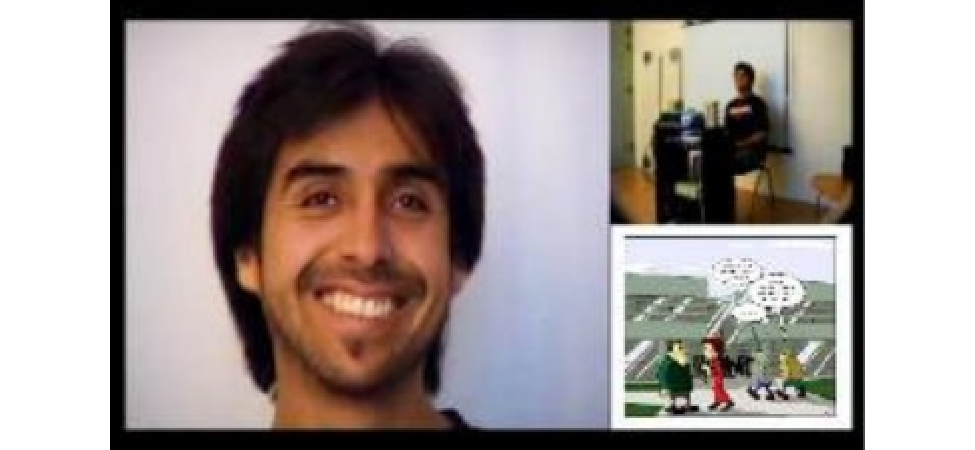
\includegraphics{ACII_2019_paper_files/figure-latex/dynemo_img-1.pdf}
\caption{\label{fig:dynemo_img}Example of a front facing recording
synced with the full view of the participant and the elicitation task.
This picture is taken from a pilot with projects collaborators and all
gave a consent for the publication of their photos and videos.}
\end{figure}

After the emotion elicitation task the encoders rated their subjective
feeling on Likert scales from 0 (``not at all'') to \nolinebreak 5
\nolinebreak (``strongly'') related to six ``basic'' emotion labels
(i.e., \emph{anger}, \emph{disgust}, \emph{fear}, \emph{happiness},
\emph{surprise} and \emph{sadness}) as well as six ``non-basic'' emotion
labels (i.e., \emph{pride}, \emph{curiosity}, \emph{boredom},
\emph{shame}, \emph{humiliation}, and \emph{disappointment}).

Finally, a debriefing session was performed to ensure that encoders were
not durably affected by the emotion elicitation task. The debriefing was
also used to check that encoders did not guess the real purpose of the
experiment (e.g.~being filmed while they were performing an emotional
elicitation task) to guarantee facial expressions' genuineness. All
encoders gave their agreement on their data and video to be processed
for research purpose only.

\hypertarget{human-facial-expression-recognition}{%
\subsection{Human Facial Expression
Recognition}\label{human-facial-expression-recognition}}

For the human facial expression recognition method, 1383
\nolinebreak student participants were recruited to annotate 232 out of
the 358 videos, therefore only the 232 annotated videos will be analysed
in this paper. Because videos have different durations, participants had
to annotate a series of video corresponding to 30min long in total. Each
video was annotated 29 times on average (\emph{SD} = 12).

The annotation of facial expressions was performed on-site using
\emph{Oudjat}, a software for designing video annotation experiments
(Dupré et al. 2015). For each video, the annotation procedure followed
two steps. First, the participants had to identify the emotional
sequences by pressing the space bar of their keyboard to indicate the
beginning and the end of the emotional sequences while watching the
video. Second, the participants watched each emotional sequence
previously identified and labeled the sequence using one of the 12
\nolinebreak emotions proposed including six ``basic'' emotion labels
(i.e., \emph{anger}, \emph{disgust}, \emph{fear}, \emph{happiness},
\emph{surprise} and \emph{sadness}) and six ``non-basic'' emotion labels
(i.e., \emph{pride}, \emph{curiosity}, \emph{boredom}, \emph{shame},
\emph{humiliation}, and \emph{disappointment}). They also had the
possibility to indicate that the sequence was expressing none of the
proposed emotion labels.

This annotation procedure results in a uni-dimensional time-series for
each video per human observer identifying for each second of the video
which emotion was recognized. Then, time-series corresponding to the
same video were aggregated to calculate the proportion of human
observers \(x_{video_{i}.label_{j}.t_{k}}\) for each second of the video
per emotional label (EQ\ref{eq:1}).

\begin{equation}
\label{eq:1}
x_{video_{i}.label_{j}.t_{k}} = \frac{n_{video_{i}.label_{j}.t_{k}}}{n_{video_{k}}}
\end{equation}

where \emph{i} is one of the 232 videos, \emph{j} is one of the six
``basic'' emotion labels, \emph{k} for each second of the video.

\hypertarget{automatic-facial-expression-recognition}{%
\subsection{Automatic Facial Expression
Recognition}\label{automatic-facial-expression-recognition}}

The 232 annotated video were processed with Affdex (SDK v3.4.1). Affdex
is an automatic facial expression recognition classifier developed and
distributed by Affectiva is a spin-off company resulting from the
research activities of MIT media lab created in 2009 (McDuff et al.
2016). Affdex's algorithm uses Histogram of Oriented Gradient (HOG)
features and Support Vector Machine (SVM) classifiers in order to
recognize facial expressions. For each video frame, Affdex identifies
the probability \(p_{video_{i}.label_{j}.t_{k}}\) from 0 to 100
(rescaled to 0 to 1 for the analysis) of the face as expressing one of
the six ``basic'' emotion labels (i.e., \emph{anger}, \emph{disgust},
\emph{fear}, \emph{happiness}, \emph{surprise} and \emph{sadness}) as
well as additional psychological states such as \emph{valence},
\emph{engagement} or \emph{contempt}, and facial features such as
\emph{cheek raise}, \emph{eye widen} or \emph{jaw drop}.

For both human and automatic recognition, to determine which of the six
``basic'' emotions can be used to identify each video, the recognition
probability for each label by frame was converted into odd ratio by
label (Dente et al. 2017). The highest sum of each odd ratio time-series
defines the label recognized by the automatic classifier (EQ\ref{eq:2}
for human recognition and EQ\ref{eq:3} for automatic recognition).
\begin{equation}
\label{eq:2}
video_{i}.label = \max\left(\frac{\sum_{k=1}^{n}x_{video_{i}.label_{j}.t_{k}}}{\sum_{k=1}^{n}x_{video_{i}.t_{k}}}\right)
\end{equation}

\begin{equation}
\label{eq:3}
video_{i}.label = \max\left(\frac{\sum_{k=1}^{f}p_{video_{i}.label_{j}.t_{k}}}{\sum_{k=1}^{f}p_{video_{i}.t_{k}}}\right)
\end{equation}

where \emph{i} is one of the 232 videos, \emph{j} is one of the six
``basic'' emotion labels, \emph{k} for each second of the \emph{n}
second video or for each frame of the \emph{f} frame video.

\hypertarget{results}{%
\section{Results}\label{results}}

Since encoders' self-reports, human annotations and the automatic
recognition include data on ``non-basic'' emotion labels and features,
the analysis is performed using only the six ``basic'' emotion labels in
order to compare them. The maximum score for self-reports, human
annotations and automatic recognition is used to label the video. In
case of more than one label obtaining the maximum value, the video is
labeled as undetermined.

\hypertarget{correlation-between-self-report-and-human-facial-expression-recognition}{%
\subsection{Correlation between self-report and human facial expression
recognition}\label{correlation-between-self-report-and-human-facial-expression-recognition}}

Encoders' subjective feeling is compared with human observers
recognition in a confusion matrix (Figure
\ref{fig:confusionMatrix_sr_hr}). Each emotion label used to describe
encoders' self-reported subjective feeling (i.e., the label rated with
the highest value) is compared with the emotion labels which were rated
with the highest score by human observers.

\begin{figure}
\centering
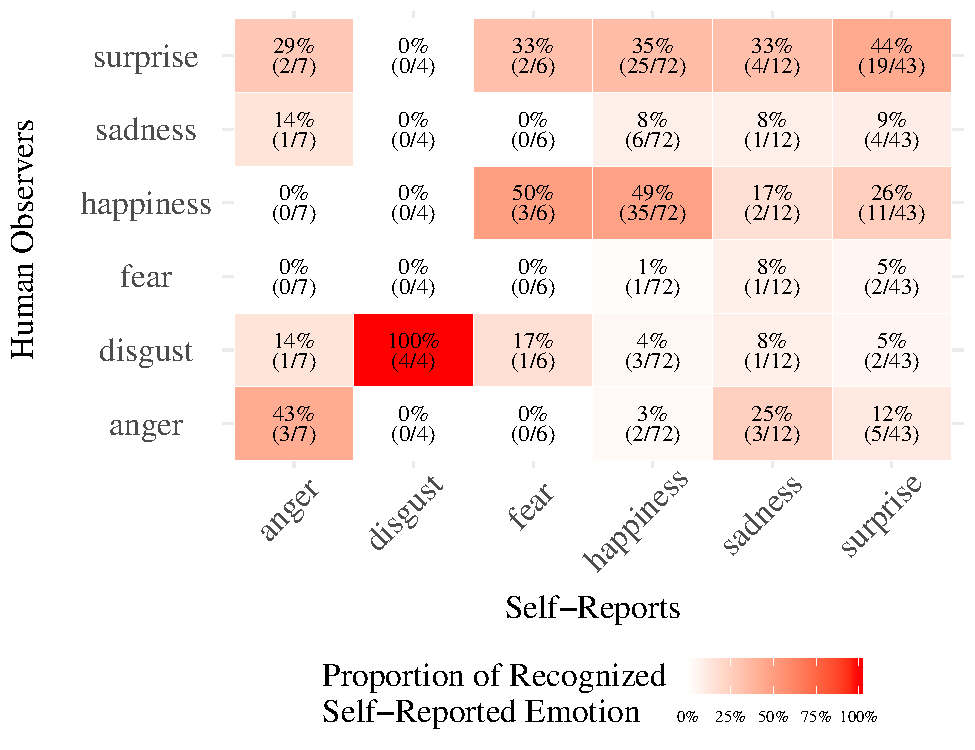
\includegraphics{ACII_2019_paper_files/figure-latex/confusionMatrix_sr_hr-1.pdf}
\caption{\label{fig:confusionMatrix_sr_hr}Confusion matrix of between
the emotion self-reported as being characteristic of the elicitation
with the emotion recognized by the human observers.}
\end{figure}

Results of the confusion matrix show a moderate agreement between the
emotion felt by the encoder during the elicitation and the emotion
recognized by the human observers (Accuracy \nolinebreak =
\nolinebreak 0.43, 95\%CI{[}0.35,0.52{]}; Kappa = 0.19) except for
\emph{disgust} (100\% of the videos self-reported). Sensitivity,
specificity, precision and F1 score for each emotion reveals that
\emph{happiness} has the highest coherence ratio whereas \emph{sadness}
has the lowest coherence ratio between true positives and false
positives (Table \ref{table:confusionTable_sr_hr}). Interestingly human
observers seem to recognize \emph{surprise} expressed in videos where
\emph{anger}, \emph{fear} \emph{happiness} and \emph{sadness} was the
highest self-reported emotion (respectively 28.6\%, 33.3\%, 34.7\% and
33.3\% of the videos self-reported), and in a lower instance
\emph{happiness} was recognized in videos where \emph{fear} and
\emph{surprise} was the highest self-reported emotion (respectively
50.0\% and 25.6\% of the videos self-reported).

\begin{table}[!h]

\caption{\label{tab:confusionTable_sr_hr}\label{table:confusionTable_sr_hr}Agreement accuracy metrics for each emotion.}
\centering
\fontsize{8}{10}\selectfont
\begin{tabu} to \linewidth {>{\raggedright}X>{\centering}X>{\centering}X>{\centering}X>{\centering}X}
\toprule
Emotion & Sensitivity & Specificity & Precision & F1\\
\midrule
anger & 0.43 & 0.93 & 0.23 & 0.3\\
disgust & 1.00 & 0.94 & 0.33 & 0.5\\
fear & 0.00 & 0.97 & 0.00 & \textit{na.}\\
happiness & 0.49 & 0.78 & 0.69 & 0.57\\
sadness & 0.08 & 0.92 & 0.08 & 0.08\\
surprise & 0.44 & 0.67 & 0.37 & 0.4\\
\bottomrule
\multicolumn{5}{l}{\textsuperscript{} Note. \textit{na.} values are produced when not enough}\\
\multicolumn{5}{l}{data are available to compute accuracy indicators.}\\
\end{tabu}
\end{table}

However, self-reports show a significant proportion of undetermined
emotional states (35.2\% of the 358 videos) which reveals the potential
limit of using 6-points likert scales to measure emotional self-reports.
Indeed, encoders can easily score to the maximum for more than one
emotion.

\hypertarget{correlation-between-self-report-and-automatic-facial-expression-recognition}{%
\subsection{Correlation between self-report and automatic facial
expression
recognition}\label{correlation-between-self-report-and-automatic-facial-expression-recognition}}

Similarly to the previous analysis, a confusion matrix was used to
compare encoders' subjective feeling with the emotion label recognized
by the automatic classifier (Figure \ref{fig:confusionMatrix_sr_ar}).

\begin{figure}
\centering
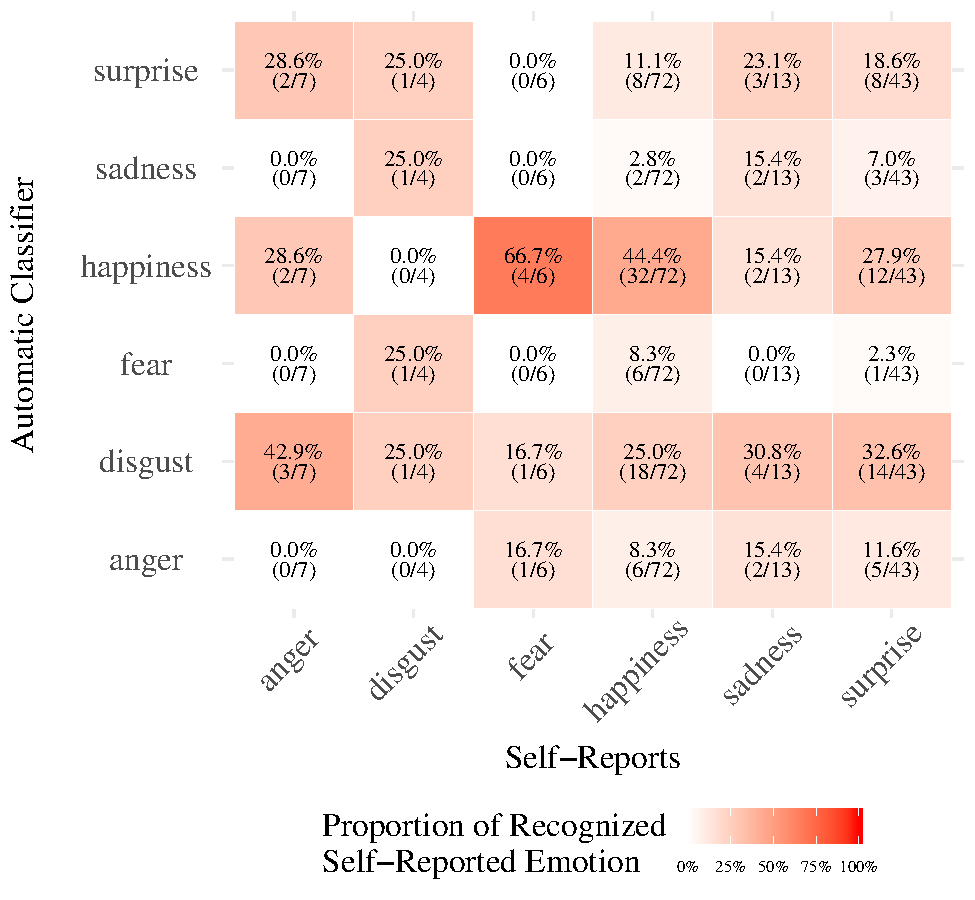
\includegraphics{ACII_2019_paper_files/figure-latex/confusionMatrix_sr_ar-1.pdf}
\caption{\label{fig:confusionMatrix_sr_ar}Confusion matrix of between
the emotion self-reported as being characteristic of the elicitation
with the emotion recognized by the automatic classifier.}
\end{figure}

Results obtained for the comparison between emotions self-reported and
recognized by the automatic classifier are somewhat similar to the ones
with human observers (Table \ref{table:confusionTable_sr_ar}). Overall,
a low agreement between emotion self-reported and emotion recognized by
the automatic classifier (Accuracy \nolinebreak = \nolinebreak 0.3,
95\%CI{[}0.22,0.38{]}; Kappa = 0.07) except for \emph{happiness} (44.4\%
of the video self-reported) is watched. Surprisingly the automatic
classifier incorrectly recognized as \emph{disgust} an important
proportion of videos in which \emph{anger}, \emph{happiness} and
\emph{surprise} was the highest self-reported emotion (respectively
42.9\%, 25.0\% and 32.6\% of the videos self-reported). In parallel, the
automatic classifier recognized as \emph{happiness} videos in which
\emph{fear} and \emph{surprise} was the highest self-reported emotion
(respectively 66.7\% and 32.6\% of the videos self-reported).

\begin{table}[!h]

\caption{\label{tab:confusionTable_sr_ar}\label{table:confusionTable_sr_ar}Agreement accuracy metrics for each emotion.}
\centering
\fontsize{8}{10}\selectfont
\begin{tabu} to \linewidth {>{\raggedright}X>{\centering}X>{\centering}X>{\centering}X>{\centering}X}
\toprule
Emotion & Sensitivity & Specificity & Precision & F1\\
\midrule
anger & 0.00 & 0.90 & 0.00 & \textit{na.}\\
disgust & 0.25 & 0.72 & 0.02 & 0.04\\
fear & 0.00 & 0.94 & 0.00 & \textit{na.}\\
happiness & 0.44 & 0.73 & 0.62 & 0.52\\
sadness & 0.15 & 0.95 & 0.25 & 0.19\\
surprise & 0.19 & 0.86 & 0.36 & 0.25\\
\bottomrule
\multicolumn{5}{l}{\textsuperscript{} Note. \textit{na.} values are produced when not enough}\\
\multicolumn{5}{l}{data are available to compute accuracy indicators.}\\
\end{tabu}
\end{table}

A comparable explanation involing the amount of undertermined video
based on self-reports can be provided as the level of undetermined
emotions are very high for the self reports.

\hypertarget{comparison-between-human-and-automatic-recognition}{%
\subsection{Comparison between human and automatic
recognition}\label{comparison-between-human-and-automatic-recognition}}

As previously mentioned, human observers appear to be more accurate than
the automatic classifier to recognize individuals' subjective feeling
(human observer Accuracy = 0.43; automatic classifier Accuracy = 0.3).
However, both make mistakes. A third confusion matrix is used to compare
similarities (diagonal) and differences between human observers and
automatic classifier in classifing the six emotion labels (Figure
\nolinebreak \ref{fig:confusionMatrix_hr_ar}).

\begin{figure}
\centering
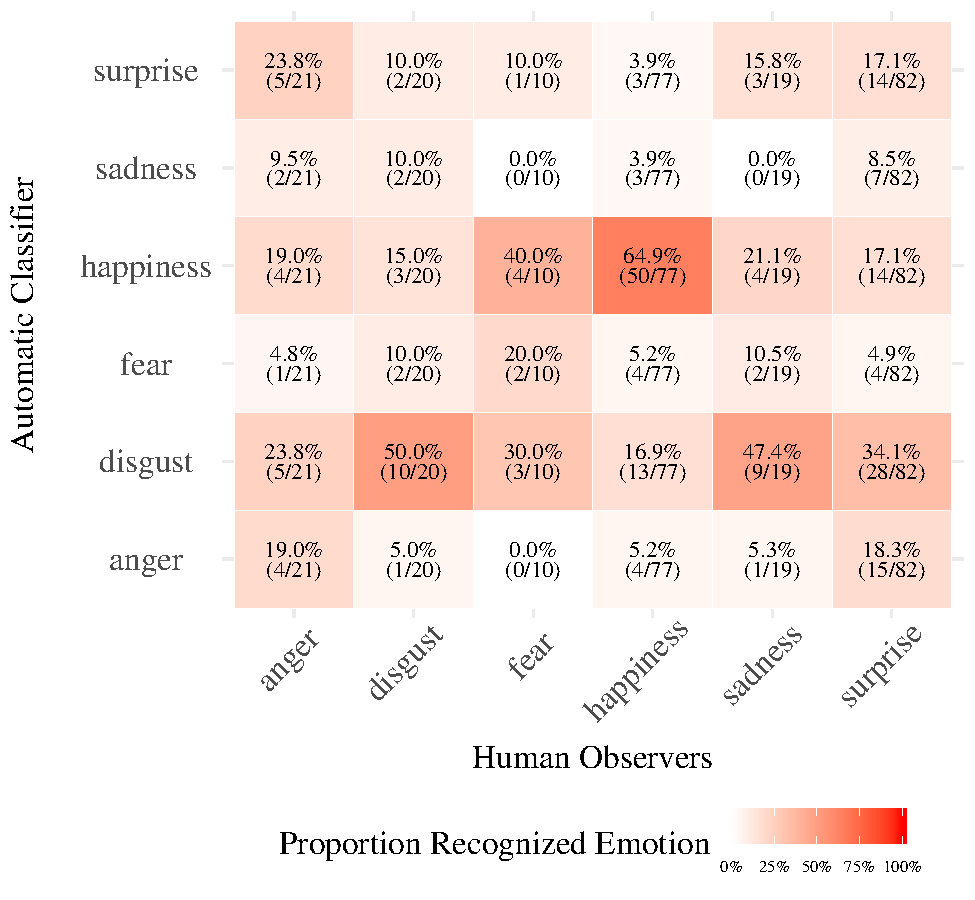
\includegraphics{ACII_2019_paper_files/figure-latex/confusionMatrix_hr_ar-1.pdf}
\caption{\label{fig:confusionMatrix_hr_ar}Proportion of emotion labels
classified by human observers which are recognized by the automatif
classifier.}
\end{figure}

The overall agreement between human observers and the automatic
classifier is in fact very low (Kappa = 0.18). Except for
\emph{happiness} and \emph{disgust} (respectively 64.9\% and 50.0\% of
common labelling), there is no clear common pattern. Moreover, the
automatic classifier has a tendency to label as \emph{disgust} videos
labeled as \emph{sadness} by human observers and as \emph{happiness}
videos labaled as \emph{fear} by human observers

\hypertarget{discussion-and-conclusion}{%
\section{Discussion and Conclusion}\label{discussion-and-conclusion}}

Despite being one on the most investigated question in affective
science, the coherence between emotion felt and facially displayed and
facial expression recognized is a hot topic. To date no clear evidence
has been found to definitely answer it. Yet, with the growing interest
of industries and government to monitor individual's psychological
states, this issue is under high pressure. The present research aims to
provide some empirical data to the question. The faces encoders
displayed when confronted with an emotional eliciting task were
submitted both to human and to automatic recognition. The criterion for
recognition accuracy was the subjective feeling self-reported by the
encoder once the elicitation task carried out. Results first reveal a
low coherence between emotion felt and facial expression displayed.
Secondly, results show a low accuracy for both humans and automatic
classifier in identifying the inner emotional states of these encoders
based on their facial expressions. Thirdly, human observers prove to be
better at recognizing the emotion facially expressed than the automatic
recognition tool is.

Such results support the hypothesis advanced by some authors of a low
emotion--expression coherence (e.g., Kappas 2003). In many instances,
facial displays are not associated with a concordant emotional state,
even any emotional state at all (Bonanno and Keltner 2004;
Fernández-Dols and Crivelli 2013). More and more evidences are showing
that facial expressions are in reality not expressing emotions (McKeown
2013). As well as other nonverbal behaviors, facial movements are not
only assumed to be determined by emotion but also by various other
causes, such as psychological states (e.g., \nolinebreak motivations or
pain), to say nothing of social context and sociocultural norms (such as
``display rules'', Ekman et al. 1987). This multiple determination
excludes any possibility of drawing an inference from facial activity on
the underlying psychological state (emotional or other). Beyond the
present observations showing a weak coherence between subjective
feelings and spontaneous facial expressions, this study provides some
light on the controversy between the behaviorist and the constructivist
approaches. The first of those two lines of thinking (Ekman 1992)
assumes that expressions of emotion are brief and coherent patterns of
facial muscle movements that co-vary with discrete subjective
experiences. Emotions and their related prototypical facial behavior are
universal because they are considered as innate mechanisms allowing
individuals to respond adaptively to evolutionary significant events
(threats, opportunities\ldots{}) encountered in the environment. Instead
of viewing emotions as natural kinds (Barrett 2017b), the constructivist
approach supposes that emotions are social constructions. The specific
emotion categories identified on the face of another person are the
result of categorization. In other words, the emotions that are
recognized by the observer are constructed in her/his mind, primarily
based on her/his conceptual knowledge of emotion. Therefore, facial
movements do not express specific emotions. It is the observer that
infers the emotional meaning of the facial expression. As a consequence,
one can predict from the first line of thinking that individuals'
emotional subjective feeling should be correlated to the recognition of
facial expressions from both human observers and automatic classifiers
whereas if emotions are social constructs, as stated by the second line
of thinking, human observer's should be better at perceiving emotions in
face than automatic classifiers. Present results plead in favor of the
latter stance. They show that human observers are more accurate than the
automatic recognition tool to identify individuals' subjective feeling
on the basis of their face. Moreover, mistakes made by human observers
look less arbitrary to the ones made by the classifier. For instance,
even if mix-up between disgust and anger is sometimes reported in
recognition studies, confusions such as the ones produced by the
classifier have never been noted for human observers. A possible
explanation is that human observers are assessing dynamic expressive
sequences. They have access to the full video which provides a kinetic
context whereas the automatic classifier only assesses the videos frame
by frame. Further research is needed to shed light on this issue.

Some limitations should be stated, notably regarding the use of
self-reports to evaluate encoders' subjective feelings. Accessing the
inner subjective feeling can be biased if not impossible. Moreover the
procedure used for human observation can also be open to dispute.
Instead of asking the human annotators to provide a unique label, a more
subtle approach was chosen to mimic results provided by the automatic
classifier . Whereas this paradigm is longer and more complicated, it
can lead to more robust results in reducing the forced-choice biais
(Russell 1993). However this procedure can also reduce the human
observers accuracy. In this regard, the results of the human observation
could have been more ambiguous because it is not the natural way that
people are inferring meaning from facial expressions. An alternative
explanation relies in reducing the recognition biais involved in the
classic recognition paradigm. Classic forced-choice paradigms obtain
artificial high results, thus by using a more evolved approach
observers' accuracy may have been lowered.

Considering the above, the results provide additional evidence that
individuals' subjective feeling can not be inferred from facial
expressions and in our case invalidate the hypothesis of hardwired
emotions unambiguously displayed on the face. Even if emotions were
hardwired, in everyday life one does not observe prototypical facial
expressions and therefore research should be focused on analysing
non-prototypical facial expressions. Advancements in identifying
``non-basic'' emotion labels (McDuff 2016) as well as non-prototypical
facial expression have been made in the developpement of automatic
facial expression recognition tools. However this result suggests that
automatic facial expression recognition tools should merely evaluate
facial morphology features such as action units (e.g., OpenFace
presented in Baltrušaitis, Robinson, and Morency 2016) rather than
inferring supposedly emotional or affective states.

\hypertarget{acknowledgment}{%
\section{Acknowledgment}\label{acknowledgment}}

The authors would like to thank Brigitte Meillon and Jean Michel Adam
who developed the software used to collect and preprocess human observer
results.

\hypertarget{references}{%
\section*{References}\label{references}}
\addcontentsline{toc}{section}{References}

\hypertarget{refs}{}
\leavevmode\hypertarget{ref-averill1980constructivist}{}%
Averill, James R. 1980. ``A Constructivist View of Emotion.'' In
\emph{Theories of Emotion}, 305--39. Elsevier.

\leavevmode\hypertarget{ref-baltruvsaitis2016openface}{}%
Baltrušaitis, Tadas, Peter Robinson, and Louis-Philippe Morency. 2016.
``Openface: An Open Source Facial Behavior Analysis Toolkit.'' In
\emph{2016 Ieee Winter Conference on Applications of Computer Vision
(Wacv)}, 1--10. IEEE.

\leavevmode\hypertarget{ref-barrett2017emotions}{}%
Barrett, Lisa Feldman. 2017a. \emph{How Emotions Are Made: The Secret
Life of the Brain}. Houghton Mifflin Harcourt.

\leavevmode\hypertarget{ref-barrett2017theory}{}%
---------. 2017b. ``The Theory of Constructed Emotion: An Active
Inference Account of Interoception and Categorization.'' \emph{Social
Cognitive and Affective Neuroscience} 12 (1): 1--23.

\leavevmode\hypertarget{ref-bonanno2004brief}{}%
Bonanno, George, and Dacher Keltner. 2004. ``Brief Report the Coherence
of Emotion Systems: Comparing `on-Line' Measures of Appraisal and Facial
Expressions, and Self-Report.'' \emph{Cognition and Emotion} 18 (3):
431--44.

\leavevmode\hypertarget{ref-crivelli2018facial}{}%
Crivelli, Carlos, and Alan J Fridlund. 2018. ``Facial Displays Are Tools
for Social Influence.'' \emph{Trends in Cognitive Sciences} 22 (5):
388--99.

\leavevmode\hypertarget{ref-darwin1872expression}{}%
Darwin, Charles. 1872. \emph{The Expression of the Emotions in Man and
Animals}. London, UK: John Murray, London UK.

\leavevmode\hypertarget{ref-dente2017measures}{}%
Dente, Pasquale, Dennis Küster, Lina Skora, and E Krumhuber. 2017.
``Measures and Metrics for Automatic Emotion Classification via Facet.''
In \emph{Proceedings of the Conference on the Study of Artificial
Intelligence and Simulation of Behaviour (Aisb)}, 160--63.

\leavevmode\hypertarget{ref-doyle2017language}{}%
Doyle, Cameron M, and Kristen A Lindquist. 2017. ``Language and Emotion:
Hypotheses on the Constructed Nature of Emotion Perception.''

\leavevmode\hypertarget{ref-dupre2015oudjat}{}%
Dupré, Damien, Daniel Akpan, Elena Elias, Jean-Michel Adam, Brigitte
Meillon, Nicolas Bonnefond, Michel Dubois, and Anna Tcherkassof. 2015.
``Oudjat: A Configurable and Usable Annotation Tool for the Study of
Facial Expressions of Emotion.'' \emph{International Journal of
Human-Computer Studies} 83: 51--61.

\leavevmode\hypertarget{ref-dupre2018accuracy}{}%
Dupré, Damien, Nicole Andelic, Gawain Morrison, and Gary McKeown. 2018.
``Accuracy of Three Commercial Automatic Emotion Recognition Systems
Across Different Individuals and Their Facial Expressions.'' In
\emph{2018 Ieee International Conference on Pervasive Computing and
Communications Workshops (Percom Workshops)}, 627--32. IEEE.

\leavevmode\hypertarget{ref-duran2017coherence}{}%
Durán, Juan I, Rainer Reisenzein, and José-Miguel Fernández-Dols. 2017.
``Coherence Between Emotions and Facial Expressions.'' \emph{The Science
of Facial Expression}, 107--29.

\leavevmode\hypertarget{ref-ekman1992argument}{}%
Ekman, Paul. 1992. ``An Argument for Basic Emotions.'' \emph{Cognition
\& Emotion} 6 (3-4): 169--200.

\leavevmode\hypertarget{ref-ekman2007directed}{}%
---------. 2007. ``The Directed Facial Action Task.'' \emph{Handbook of
Emotion Elicitation and Assessment} 47: 53.

\leavevmode\hypertarget{ref-ekman1987universals}{}%
Ekman, Paul, Wallace V Friesen, Maureen O'sullivan, Anthony Chan, Irene
Diacoyanni-Tarlatzis, Karl Heider, Rainer Krause, et al. 1987.
``Universals and Cultural Differences in the Judgments of Facial
Expressions of Emotion.'' \emph{Journal of Personality and Social
Psychology} 53 (4): 712.

\leavevmode\hypertarget{ref-ekman1988universality}{}%
Ekman, Paul, and Karl G Heider. 1988. ``The Universality of a Contempt
Expression: A Replication.'' \emph{Motivation and Emotion} 12 (3):
303--8.

\leavevmode\hypertarget{ref-fernandez2013emotion}{}%
Fernández-Dols, José-Miguel, and Carlos Crivelli. 2013. ``Emotion and
Expression: Naturalistic Studies.'' \emph{Emotion Review} 5 (1): 24--29.

\leavevmode\hypertarget{ref-fridlund1995human}{}%
Fridlund, Alan J, and Erika L Rosenberg. 1995. ``Human Facial
Expression: An Evolutionary View.'' \emph{Nature} 373 (6515): 569--69.

\leavevmode\hypertarget{ref-frijda1997facial}{}%
Frijda, Nico H, and Anna Tcherkassof. 1997. ``Facial Expressions as
Modes of Action Readiness.'' \emph{The Psychology of Facial Expression},
78--102.

\leavevmode\hypertarget{ref-kappas2003facial}{}%
Kappas, Arvid. 2003. ``What Facial Activity Can and Cannot Tell Us About
Emotions.'' In \emph{The Human Face}, 215--34. Springer.

\leavevmode\hypertarget{ref-kraut1979social}{}%
Kraut, Robert E, and Robert E Johnston. 1979. ``Social and Emotional
Messages of Smiling: An Ethological Approach.'' \emph{Journal of
Personality and Social Psychology} 37 (9): 1539.

\leavevmode\hypertarget{ref-lindquist2013s}{}%
Lindquist, Kristen A, and Maria Gendron. 2013. ``What's in a Word?
Language Constructs Emotion Perception.'' \emph{Emotion Review} 5 (1):
66--71.

\leavevmode\hypertarget{ref-mcduff2016discovering}{}%
McDuff, Daniel. 2016. ``Discovering Facial Expressions for States of
Amused, Persuaded, Informed, Sentimental and Inspired.'' In
\emph{Proceedings of the 18th Acm International Conference on Multimodal
Interaction}, 71--75. ACM.

\leavevmode\hypertarget{ref-mcduff2016affdex}{}%
McDuff, Daniel, Abdelrahman Mahmoud, Mohammad Mavadati, May Amr, Jay
Turcot, and Rana el Kaliouby. 2016. ``AFFDEX Sdk: A Cross-Platform
Real-Time Multi-Face Expression Recognition Toolkit.'' In
\emph{Proceedings of the 2016 Chi Conference Extended Abstracts on Human
Factors in Computing Systems}, 3723--6. ACM.

\leavevmode\hypertarget{ref-mckeown2013analogical}{}%
McKeown, Gary J. 2013. ``The Analogical Peacock Hypothesis: The Sexual
Selection of Mind-Reading and Relational Cognition in Human
Communication.'' \emph{Review of General Psychology} 17 (3): 267--87.

\leavevmode\hypertarget{ref-niedenthal2017embodied}{}%
Niedenthal, Paula M, Adrienne Wood, Magdalena Rychlowska, and Sebastian
Korb. 2017. ``Embodied Simulation in Decoding Facial Expression.''
\emph{The Science of Facial Expression}, 397.

\leavevmode\hypertarget{ref-russell1993forced}{}%
Russell, James A. 1993. ``Forced-Choice Response Format in the Study of
Facial Expression.'' \emph{Motivation and Emotion} 17 (1): 41--51.

\leavevmode\hypertarget{ref-tcherkassof2013dynemo}{}%
Tcherkassof, Anna, Damien Dupré, Brigitte Meillon, Nadine Mandran,
Michel Dubois, and Jean-Michel Adam. 2013. ``DynEmo: A Video Database of
Natural Facial Expressions of Emotions.'' \emph{The International
Journal of Multimedia \& Its Applications} 5 (5): 61--80.

\leavevmode\hypertarget{ref-de2019mama}{}%
Waal, Frans de. 2019. \emph{Mama's Last Hug: Animal Emotions and What
They Teach Us About Ourselves}. Granta Books.

\end{document}


